\section{Band Reject}
\subsection{Setup}


\begin{figure}[h]
    \centering
    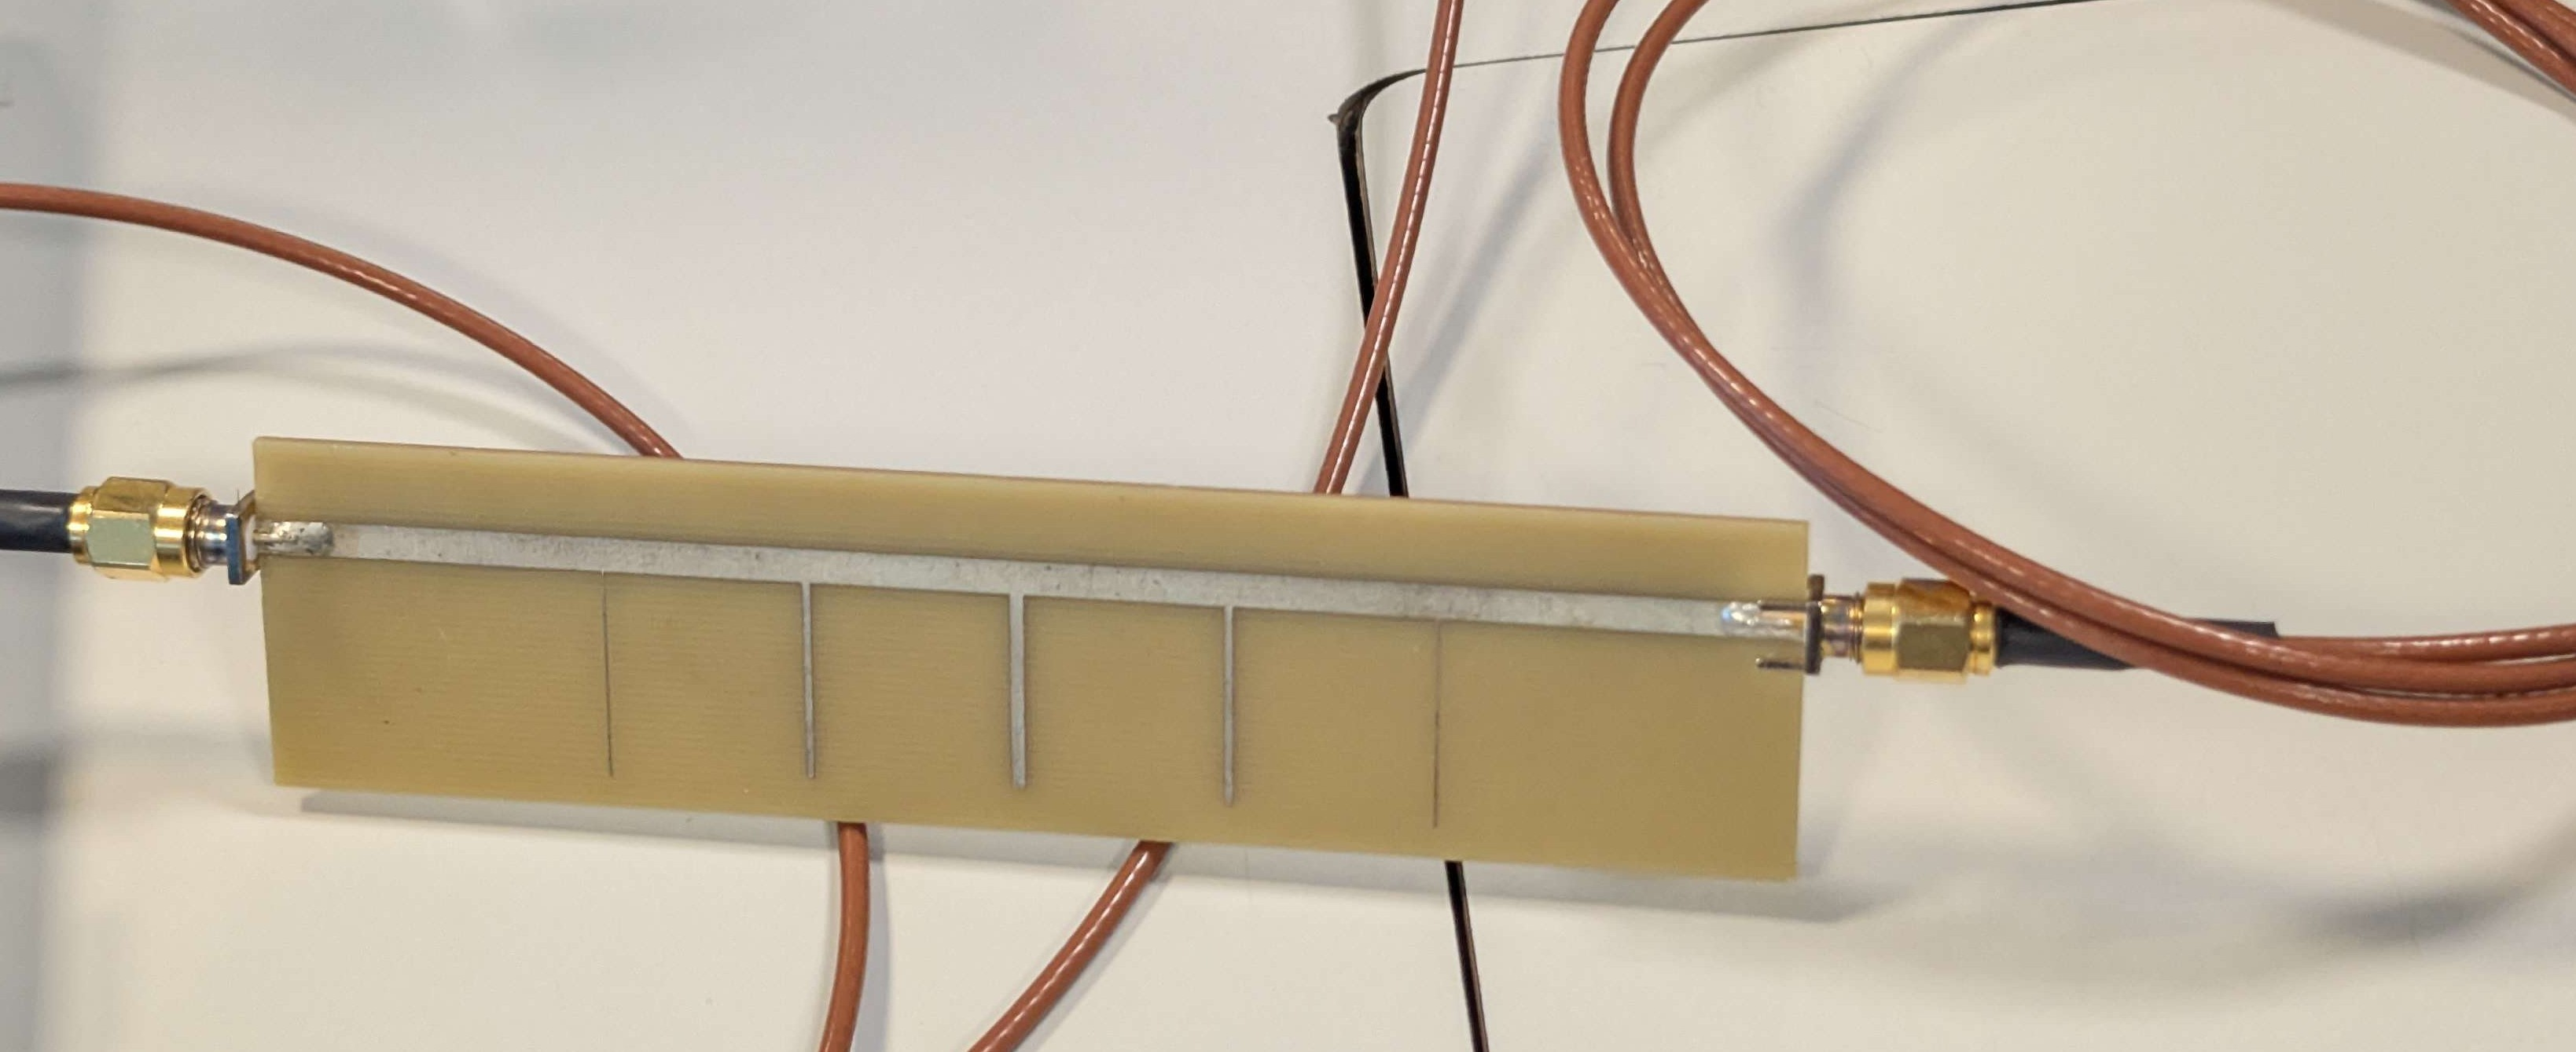
\includegraphics[width=0.5\textwidth]{Band Reject/Plots/BR_photo.jpg}
    \caption{Band reject device under test}
    \label{fig:device}
\end{figure}


\subsection{Analysis of the measurement}

For this device, the plot of the magnitude of the S-matrix covers all the investigated frequency range. This is because the behaviour of the DUT has to be analyzed over a wide frequency band. As a consequence, in Fig.~(9) the frequency is reported in GHz.

\begin{figure}[h]
    \centering

    \begin{minipage}{0.48\textwidth}
        \centering
        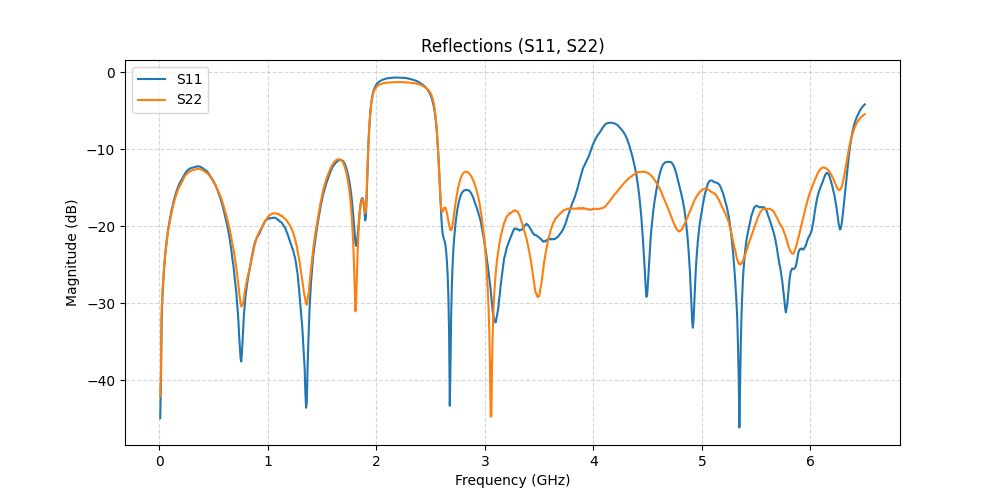
\includegraphics[width=\textwidth]{Band Reject/Plots/BR_reflections.png}
        \caption{Reflection coefficients S11 and S22}
        \label{fig:reflections}
    \end{minipage}
    \hfill
    \begin{minipage}{0.48\textwidth}
        \centering
        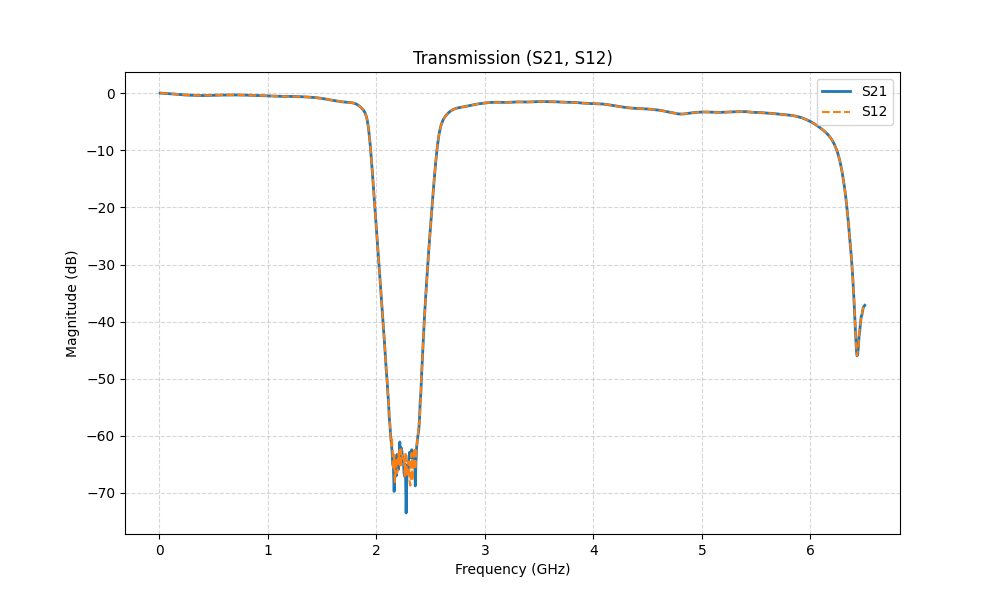
\includegraphics[width=\textwidth]{Band Reject/Plots/BR_trasmission.png}
        \caption{Transmission coefficients S21 and S12}
        \label{fig:transmission}
    \end{minipage}

\end{figure}

The first thing to observe from the plot is that the DUT is passive and (approximately) symmetric, so the behavior is independent of which port is used for transmission. 

Then, by observing the transmission plot of S21/S12, we can notice that both at high frequency and at low frequency there is good transmissivity, with the magnitude close to 0 dB, except at a specific frequency where the transmissivity strongly decreases.

\begin{table}[h]
\centering
\begin{tabular}{|c|c|c|c|}
\hline
\textbf{Parametro} & \textbf{Freq (GHz)} & \textbf{Min Magn (dB)} & \textbf{BW (GHz)} \\ \hline
\textbf{S12}       & 2.3140              & -68.69                 & 0.8048            \\ \hline
\textbf{S21}       & 2.2750              & -73.50                 & 0.8048            \\ \hline
\end{tabular}
\caption{Parametri di trasmissione S12 e S21}
\label{tab:parametri_s}
\end{table}

With the data processing, we can find the value of the frequency at which the strongest attenuation occurs for both S21 and S12 parameters, reported in Tab.~(2). The very low value of about -75 dB guarantees that the signal is almost completely suppressed at that frequency. This is also confirmed by looking at the reflection coefficients S11 and S22, where a peak occurs at the same frequency.
The -3 dB bandwidth was estimated to be about 0.8 GHz, corresponding to the frequency region that is not transmitted by the DUT.
